
\documentclass{beamer} %
\usetheme{Madrid}
%\usecolortheme{spruce}
% temas disponíveis:  default, structure, Sidebartab,beetle, crane, dove,fly, monarca, seagull, wolverine, beaver, spruce

%você pode consultar as ores disponíveis  nessa interessante matriz de cores e temas, disponível em: https://mpetroff.net/files/beamer-theme-matrix/
\usepackage[utf8]{inputenc}
\usepackage[portuguese]{babel}
\usepackage{times}
\usepackage{verbatim}
\usepackage[style=ieee]{biblatex}
\setbeamertemplate{bibliography item}{\insertbiblabel}

\usepackage{filecontents}
\begin{filecontents*}{\jobname.bib}
@book{knuth,
  author       = {Knuth, Donald E.},
  title        = {The {\TeX} book},
  date         = 1984,
  maintitle    = {Computers \& Typesetting},
  volume       = {A},
  publisher    = {Addison-Wesley},
  location     = {Reading, Mass.},
  langid       = {english},
  langidopts   = {variant=american},
  sortyear     = {1984-1},
  sorttitle    = {Computers & Typesetting A},
  indexsorttitle= {The TeXbook},
  indextitle   = {\protect\TeX book, The},
  shorttitle   = {\TeX book}
}

@article{einstein,
    author = {Einstein, A.},
    title = {Die Grundlage der allgemeinen Relativitätstheorie},
    journal = {Annalen der Physik},
    volume = {354},
    number = {7},
    doi = {10.1002/andp.19163540702},
    pages = {769--822},
    year = {1916}
}
\end{filecontents*}
\addbibresource{\jobname.bib}



\author[Lara, Wellington] % (optional, for multiple authors)
{Lara Marinelli \and Wellington Martins}
%{Lara Marinelli\inst{1} \and Wellington Martins\inst{2}}
    \title[PPA Day]{Como utilizar o Beamer e o Overleaf\footnote{https://www.overleaf.com/} para ganhar tempo em suas apresenta\c{c}\~{o}es?}
    
\begin{comment}    
\institute[VFU] % (optional)
{
  \inst{1}%
  Faculty of Physics\\
  Very Famous University
  \and
  \inst{2}%
  Faculty of Chemistry\\
  Very Famous University
}
\end{comment}
\begin{document}

\begin{comment}
:Title: Beamer arrows
:Tags: Remember picture, Beamer, Physics & chemistry, Overlays
:Use page: 3

With PGF/TikZ version 1.09 and later, it is possible to draw paths between nodes across
different pictures. This is a useful feature for presentations with the
Beamer package. In this example I've combined the new PGF/TikZ's overlay feature
with Beamer overlays. Download the PDF version to see the result.

**Note.** This only works with PDFTeX, and you have to run PDFTeX twice.

| Author: Kjell Magne Fauske

\end{comment}

\frame{\titlepage}

\begin{frame}
\frametitle{Por que você precisa saber que o Beamer existe?}
\begin{itemize}
    \item Material visual de qualidade para as apresentações
    \item Otimização de tempo
    \item Foco no conteúdo
\end{itemize}
\end{frame}


\begin{frame}
\frametitle{Você pode querer começar a sua apresentação com as várias partes da exposição}
\tableofcontents
\end{frame}

\section{Introdução}
\begin{frame}
\frametitle{Você tem algo muito importante a dizer}

Talvez você precise \alert{destacar} algumas definições e exemplos. Use o destaque com sabedoria.

\begin{block}{Conceito}
textos essenciais
\end{block}

\begin{alertblock}{Definição}
textos essenciais
\end{alertblock}

\end{frame}

\section{Metodologia}
\begin{frame}
\frametitle{Para explicar como fez...}
Você pode precisar mostrar alguns dados..
\begin{table}
\begin{tabular}{l | c | c | c | c } 
Cidade & Observação & Observação 2 & Observação 3 & Total \\
\hline \hline
São Paulo & 13:04 & 24:15 & 18:34 & 55:53 \\ 
Rio de Janeiro & 8:00 & 22:45 & 23:02 & 53:47\\
Porto Alegre & 14:00 & 28:00 & n/a & n/a\\
Minas Gerais & 9:22 & 21:10 & 24:03 & 54:35 
\end{tabular}
\caption{Medições de exemplo}
\end{table}
\end{frame}

\begin{frame}
\frametitle{ou talvez precise ilustrar}
\begin{figure}
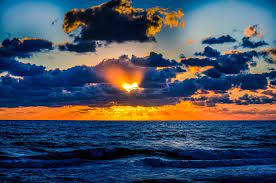
\includegraphics[scale=0.5]{exemplo.jpg}
\caption{legenda}
\end{figure}

\end{frame}





\begin{frame}{ou você pode precisar explicar item a item}
\begin{itemize}
\item<+-> parte 1
\item<+-> parte 2
\item<+-> parte 3
\item<+-> parte 4
\end{itemize}
\end{frame}

\section{Considerações finais}
\begin{frame}
    Ao longo da sua apresentação, provavelmente terão algumas citações, por exemplo \cite{einstein}  e \cite{knuth}.
\end{frame} 


\begin{frame}{Considerações finais}
Esperamos ter te convencido a experimentar o Beamer.
Com o conteúdo que vimos aqui, você pode ter uma base para construir a sua apresentação.
Vamos para a parte prática!
    
\end{frame}


\begin{frame}
\frametitle{Referências bibliográficas}
\printbibliography
\end{frame}

\end{document}
